\begin{exercise}{Maille de l'argent}{1}{Sup}
{Cristalographie}{bermu}

L’argent cristallise dans un système cfc de paramètre $a = 408.6$ pm.

\begin{questions}
    \question Représenter schématiquement la maille de l'argent.
    \question Quelle est la valeur du rayon atomique de l’argent en supposant le cristal compact ?
\end{questions}
\end{exercise}

\begin{solution}
    \begin{questions}
        \question ~
        \question 
    \end{questions}
\end{solution}


%%%%%%%%%%%%%%%%%%%%%%%%%%%%%%%%%%%%%%%%%%%%%%%%%%%%%%%%%%%%%%%%%%%%%%%%%%%%%%%%%%%%%%%%%%%%%%%%%


\begin{exercise}{Variétés allotropiques du fer}{1}{Sup}
{Cristalographie,Variétés allotropiques}{bermu}

Le fer peut cristalliser suivant deux variétés allotropiques :
\begin{itemize}
    \item Fe$_\alpha$ : structure Cubique Centrée (CC), stable à basse température ;
    \item Fe$_\gamma$ : structure Cubique Faces Centrées (CFC), stable à haute température.
\end{itemize}

\noindent Pour chacune des deux structures :
\begin{questions}
    \question Représenter schématiquement la maille de chacun des deux réseaux.
    \question Préciser la coordinence et la population.
    \question Exprimer le rayon atomique du fer.
    \question Calculer la compacité de la structure ; lequel est le plus compact ?
    \question Exprimer la masse volumique des deux variétés.
\end{questions}

\paragraph{Données}
\begin{itemize}
    \item paramètre de maille du fer $\alpha$ : $a_\alpha = 291$ pm ;
    \item paramètre de maille du fer $\gamma$ : $a_\gamma = 365$ pm ;
    \item masse molaire du fer $M_\text{Fe} = 55,85~\mathrm{g\cdot mol^{-1}}$ ;
    \item nombre d'Avogadro $\cal{N}_\textsc{a} = 6,022\times 10^{23}~\mathrm{mol^{-1}}$ ;
\end{itemize}
\end{exercise}

\begin{solution}
    \begin{questions}
        \question ~
        \question (CC$\alpha$) Coordinence 8, Population 2 (CFC$\gamma$) Coordinence 12, Population 4
        \question (CC$\alpha$)$r_\alpha = \dfrac{\sqrt{3}}{4} a_\alpha = 126$ pm, (CFC$\gamma$)  $r_\gamma = \dfrac{\sqrt{2}}{4} a_\alpha = 129$ pm
        \question  (CC$\alpha$) 68\% (CFC$\gamma$) 74\%
        \question  (CC$\alpha$) 7530 $\mathrm{kg\cdot m^{-3}}$ (CFC$\gamma$) 7630 $\mathrm{kg\cdot m^{-3}}$
    \end{questions}
\end{solution}

%%%%%%%%%%%%%%%%%%%%%%%%%%%%%%%%%%%%%%%%%%%%%%%%%%%%%%%%%%%%%%%%%%%%%%%%%%%%%%%%%%%%%%%%%%%%%%%%%


\begin{exercise}{Stockage sous forme d'hydrures}{1}{Sup}
{Cristalographie,Alliages de substitution, Alliages d'insersion}{bermu}

Le dihydrogène peut être stocké dans les métaux sous forme d'hydrures métalliques. On étudie le processus de stockage
$$\mathrm{FeTi_{(s)} + \frac{\mathit{x}}{2} H_{2(g)} = FeTiH_{\mathit{x}(s)}},$$
$\mathit{x}$ étant un nombre stoechiométrique à déterminer.

L'alliage FeTi$_\mathrm{(s)}$ est une structure cubique simple comportant un atome de titane sur chaque sommet et un atome de fer au centre. Un atome d'hydrogène peut se placer dans les sites octaédriques de la maille métallique.

\begin{questions}
    \question Quel est le type d'alliage de FeTi ? Qu'en est-il lorsqu'il y a absorption d'hydrogène ?
    \question Représenter la maille de FeTi$_\mathrm{(s)}$ ainsi qu'un site octaédrique.
    \question Donner la population et la coordinence de chaque atome : Fe et Ti en l'absence d'hydrogène et H en supposant que tous les sites sont occupés. En déduire $\mathit{x}$.
    \question Donner le rayon d'habitabilité maximale du site intersticiel O. Est-ce cohérent avec les données ?
    \question En réalité, $\mathit{x} = 1,9$. Calculer la capacité volumique d'absorption de H$_2$ par FeTi en kg d'hydrogène par m$^3$ de FeTi.
\end{questions}

\paragraph{Données}
\begin{itemize}
    \item rayons atomiques : $r_\text{H} = 25$ pm / $r_\text{Fe} = r_\text{Ti} = 140$ pm ;
    \item paramètre de maille de FeTi $\gamma$ : $a = 298$ pm ;
    \item distance H--H dans H$_{2\text{(g)}}$ : $d_\text{H---H} = 74$ pm ;
    \item masse molaires (en $\mathrm{g\cdot mol^{-1}}$) : $\text{H} = 1,0$, $\text{Ti} = 47,9$, $\text{Fe} = 55,8$ ; 
    \item nombre d'Avogadro $\cal{N}_\textsc{a} = 6,022\times 10^{23}~\mathrm{mol^{-1}}$ ;
\end{itemize}
\end{exercise}

\begin{solution}
\begin{questions}
    \question Alliage de substitution pour FeTi avec insertion de H$_2$.
    \question ~
    \question Population : 1 Fe, 1 Ti, 3 H, Coordinences : Fe 8, Ti 8, H 4.
    \question $r = \dfrac{\sqrt{2}}{2}a - r_\text{Ti} = 71$ pm vs $r_\text{H} = 25$ pm et $d_\text{H---H} = 74$ pm.
    \question $\dfrac{\mathit{x} M_\text{H}}{\cal{N}_\textsc{a} a^3} = 112 \mathrm{kg\cdot m^{-3}}$.
\end{questions}
\end{solution}

%%%%%%%%%%%%%%%%%%%%%%%%%%%%%%%%%%%%%%%%%%%%%%%%%%%%%%%%%%%%%%%%%%%%%%%%%%%%%%%%%%%%%%%%%%%%%%%%%


\begin{exercise}{Semi-conducteurs}{1}{Sup}
{Cristalographie,Solides macrovalents}{bermu}

L'arséniure de gallium (AsGa) est un composé de la famille des semi-conducteurs III-V très utilisés en électronique. Sa structure est une maille cubique face centrée pour As avec occupation de 1 site tétraédrique sur 2 pour Ga.

\begin{questions}
    \question Représenter la maille de AsGa.
    \question Quelle est la population et la coordinence de la maille.
    \question Montrer que le rapport des rayons ioniques vérifie une condition que l'on donnera. Cela est-il cohérent avec la valeur du paramètre de maille ?
    \uplevel{L'AsGa est produit par épitaxie entre le gallium et le triiodure d'arsenic AsI$_3$ :
    $$\mathrm{2 Ga + 2 AsI_3 \longrightarrow 2 AsGa + 3 I_2}.$$
    }
    \question Quels types de solides sont ces espèces chimiques ?
\end{questions}

\paragraph{Données}
\begin{itemize}
    \item rayons ioniques : $r_\text{As} = 230$ pm, $r_\text{Ga} = 61$ pm ;
    \item paramètre de maille de AsGa $\gamma$ : $a = 565$ pm ;
    \item masse molaires (en $\mathrm{g\cdot mol^{-1}}$) : $\text{As} = 74.9$, $\text{Ga} = 69.7$ ; 
    \item nombre d'Avogadro $\cal{N}_\textsc{a} = 6,022\times 10^{23}~\mathrm{mol^{-1}}$ ;
\end{itemize}

\begin{figure}[H]
    \centering
    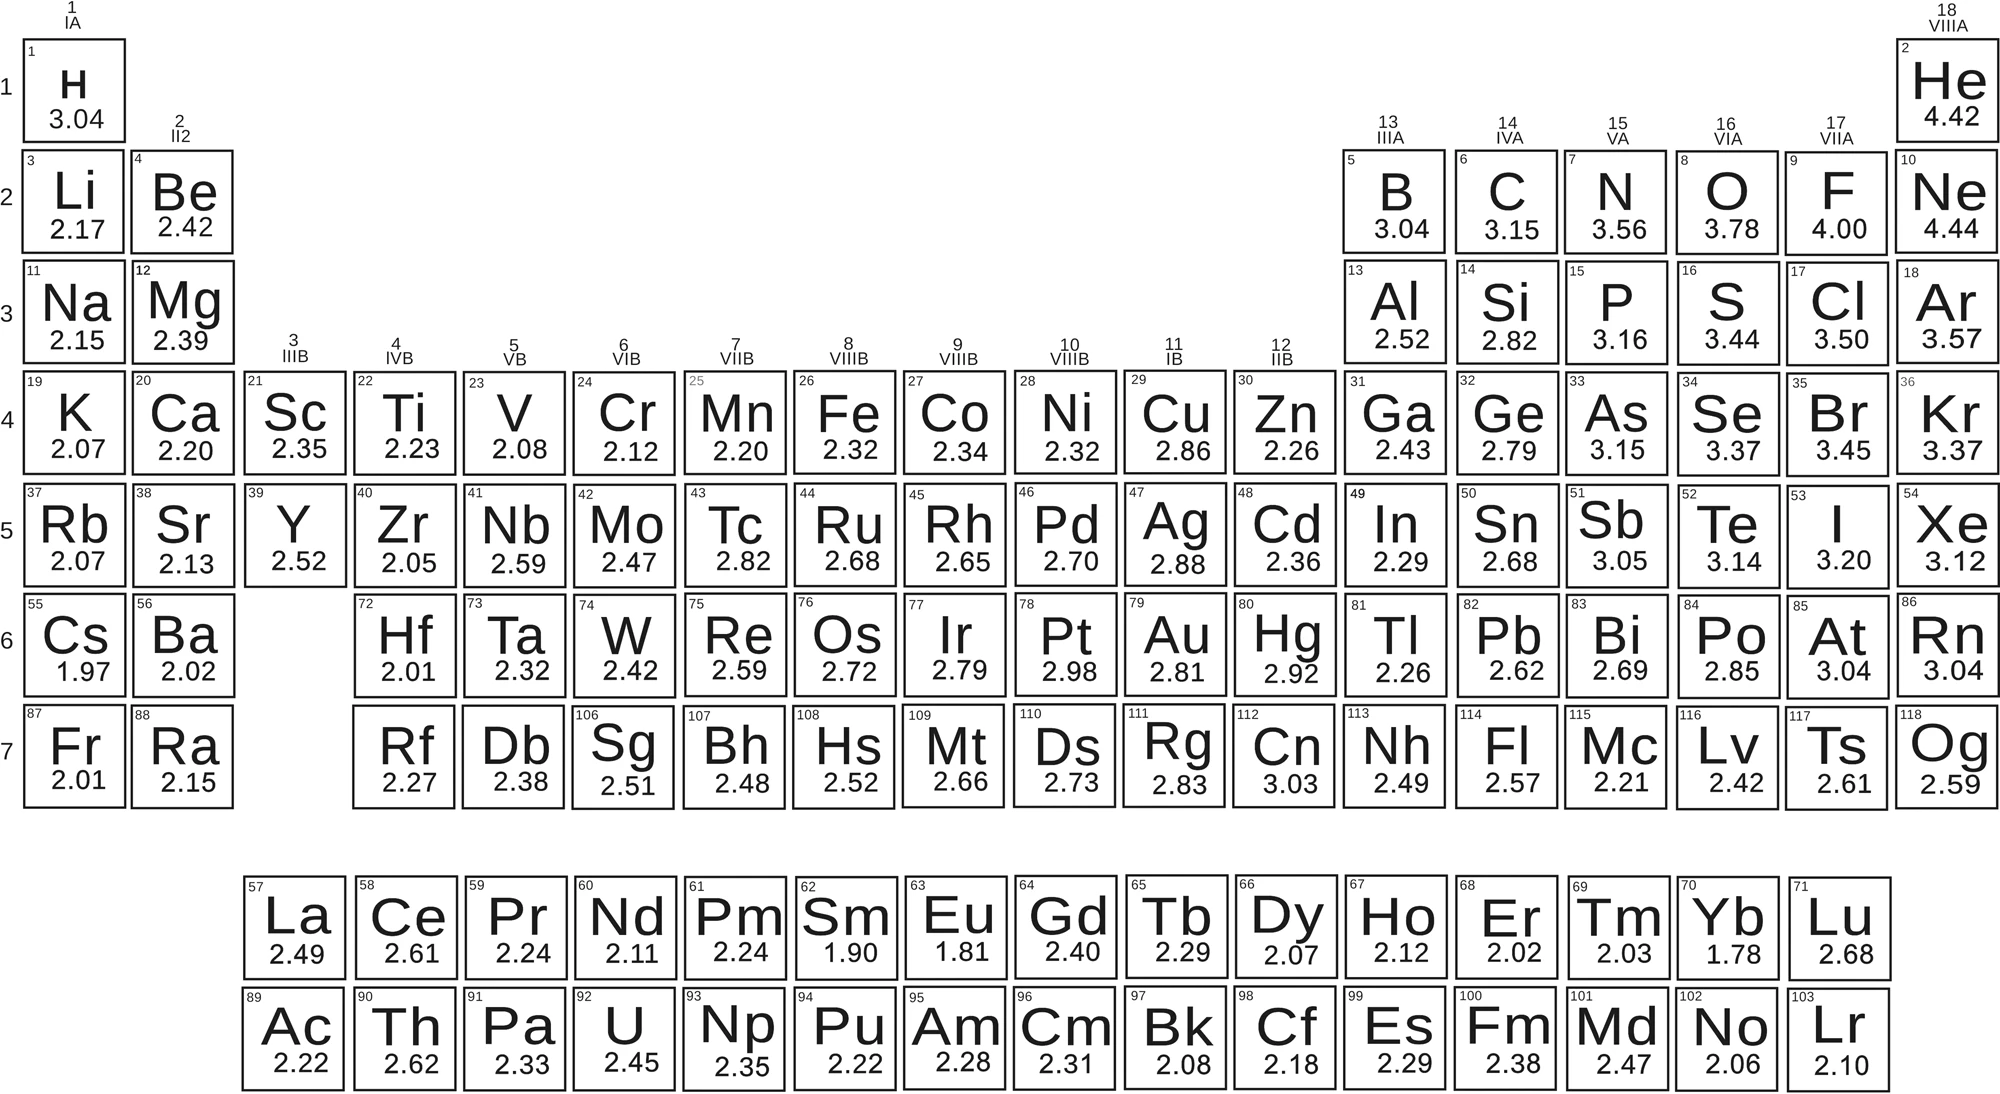
\includegraphics[width=\linewidth]{chimie/cristallo/electroneg_mulliken.png}
    \caption{Table périodique des électronégativités des éléments dans l'échelle de Mulliken.}
\end{figure}
\end{exercise}

\begin{solution}
\begin{questions}
    \question ~\\[0em] 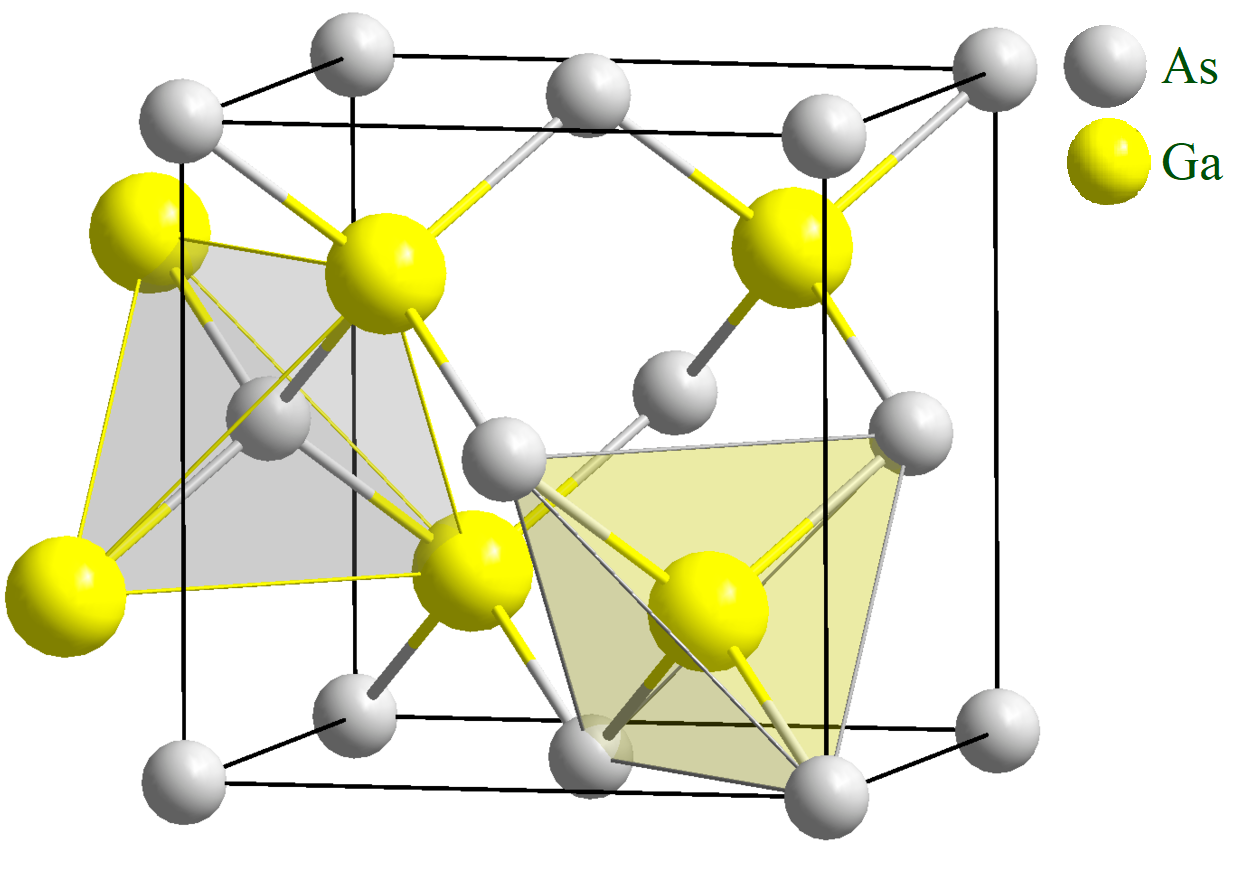
\includegraphics[width=0.45\linewidth]{chimie/cristallo/AsGa.png}
    \question Population 4 As $+$ 4 Ga, Coordinence 8 pour CFC, 4 pour As et Ga.
    \question $r_\text{Ga}/r_\text{As} > \sqrt{3/2} - 1 \simeq 0.225$.\\
    (\'Ealement $r_\text{Ga}/r_\text{As} < \sqrt{2}-1 \simeq 0.414$, l'autre maille étant NaC$\ell$, CFC insertion octaédrique)
    \question Ga : solide métallique, AsI$_3$ solide ionique, AsGa est un semi-métal, I$_2$ solide moléculaire
\end{questions}
\end{solution}